\section{Scenario and challenges}
\label{sec:scenario}

\ac{SCITE} is designed for the following scenario: A physician has been able to extract tumor tissue from a patient, either through surgery or other methods. Then, individual cells are extracted from the tissue, their genome is sequenced, and the resulting sequence of base pairs is scanned for subsequences, so-called genes. These genes may either be present in their most common form or in a less common, mutated way. The scanner identifies these mutations and produces a mutation matrix with an entry for every cell-gene combination, where 1 denotes that the cell has this mutation and 0 denotes the opposite. This matrix itself may already be interesting to evaluate, but it should be handled with caution since, as stated before, the process of amplifying and sequencing the genome is very prone to errors. While there is often only a small chance to identify a mutation where there isn't one (false positives), there is a high chance to miss a mutation (false negative). Lastly, there is also a high chance that genes are simply lost in the process. In this case, the matrix contains a third ``unknown'' entry encoded as 2. Jahn et al. \cite{tree2016} quote one example with a probability for false positives of $6.04 \cdot 10^{-}$, a probability for false negatives of $0.4309$, and a probability for missing data of $0.45$.

It is however possible to catch some of these errors with some assumptions on how mutations are introduced to the tumor: First of all, we assume that there are no mutations in the observed genes outside of the tumor. This means that before the tumor came into existence, there were only perfectly normal cells. When a cell replicates itself, it creates a perfect copy of its genome for one of the two new cells, and these two cells pass their genome to their subclones too. However, cells can not share or swap their genome. If a gene of a cell's genome mutates, the altered genome will therefore be passed down to its subclones and its subclones only. If we then also assume that every gene only mutates once in the whole history of the tumor (the so-called infinite sites assumption), we can arrange the mutations in their order of occurrence.

\begin{figure}
    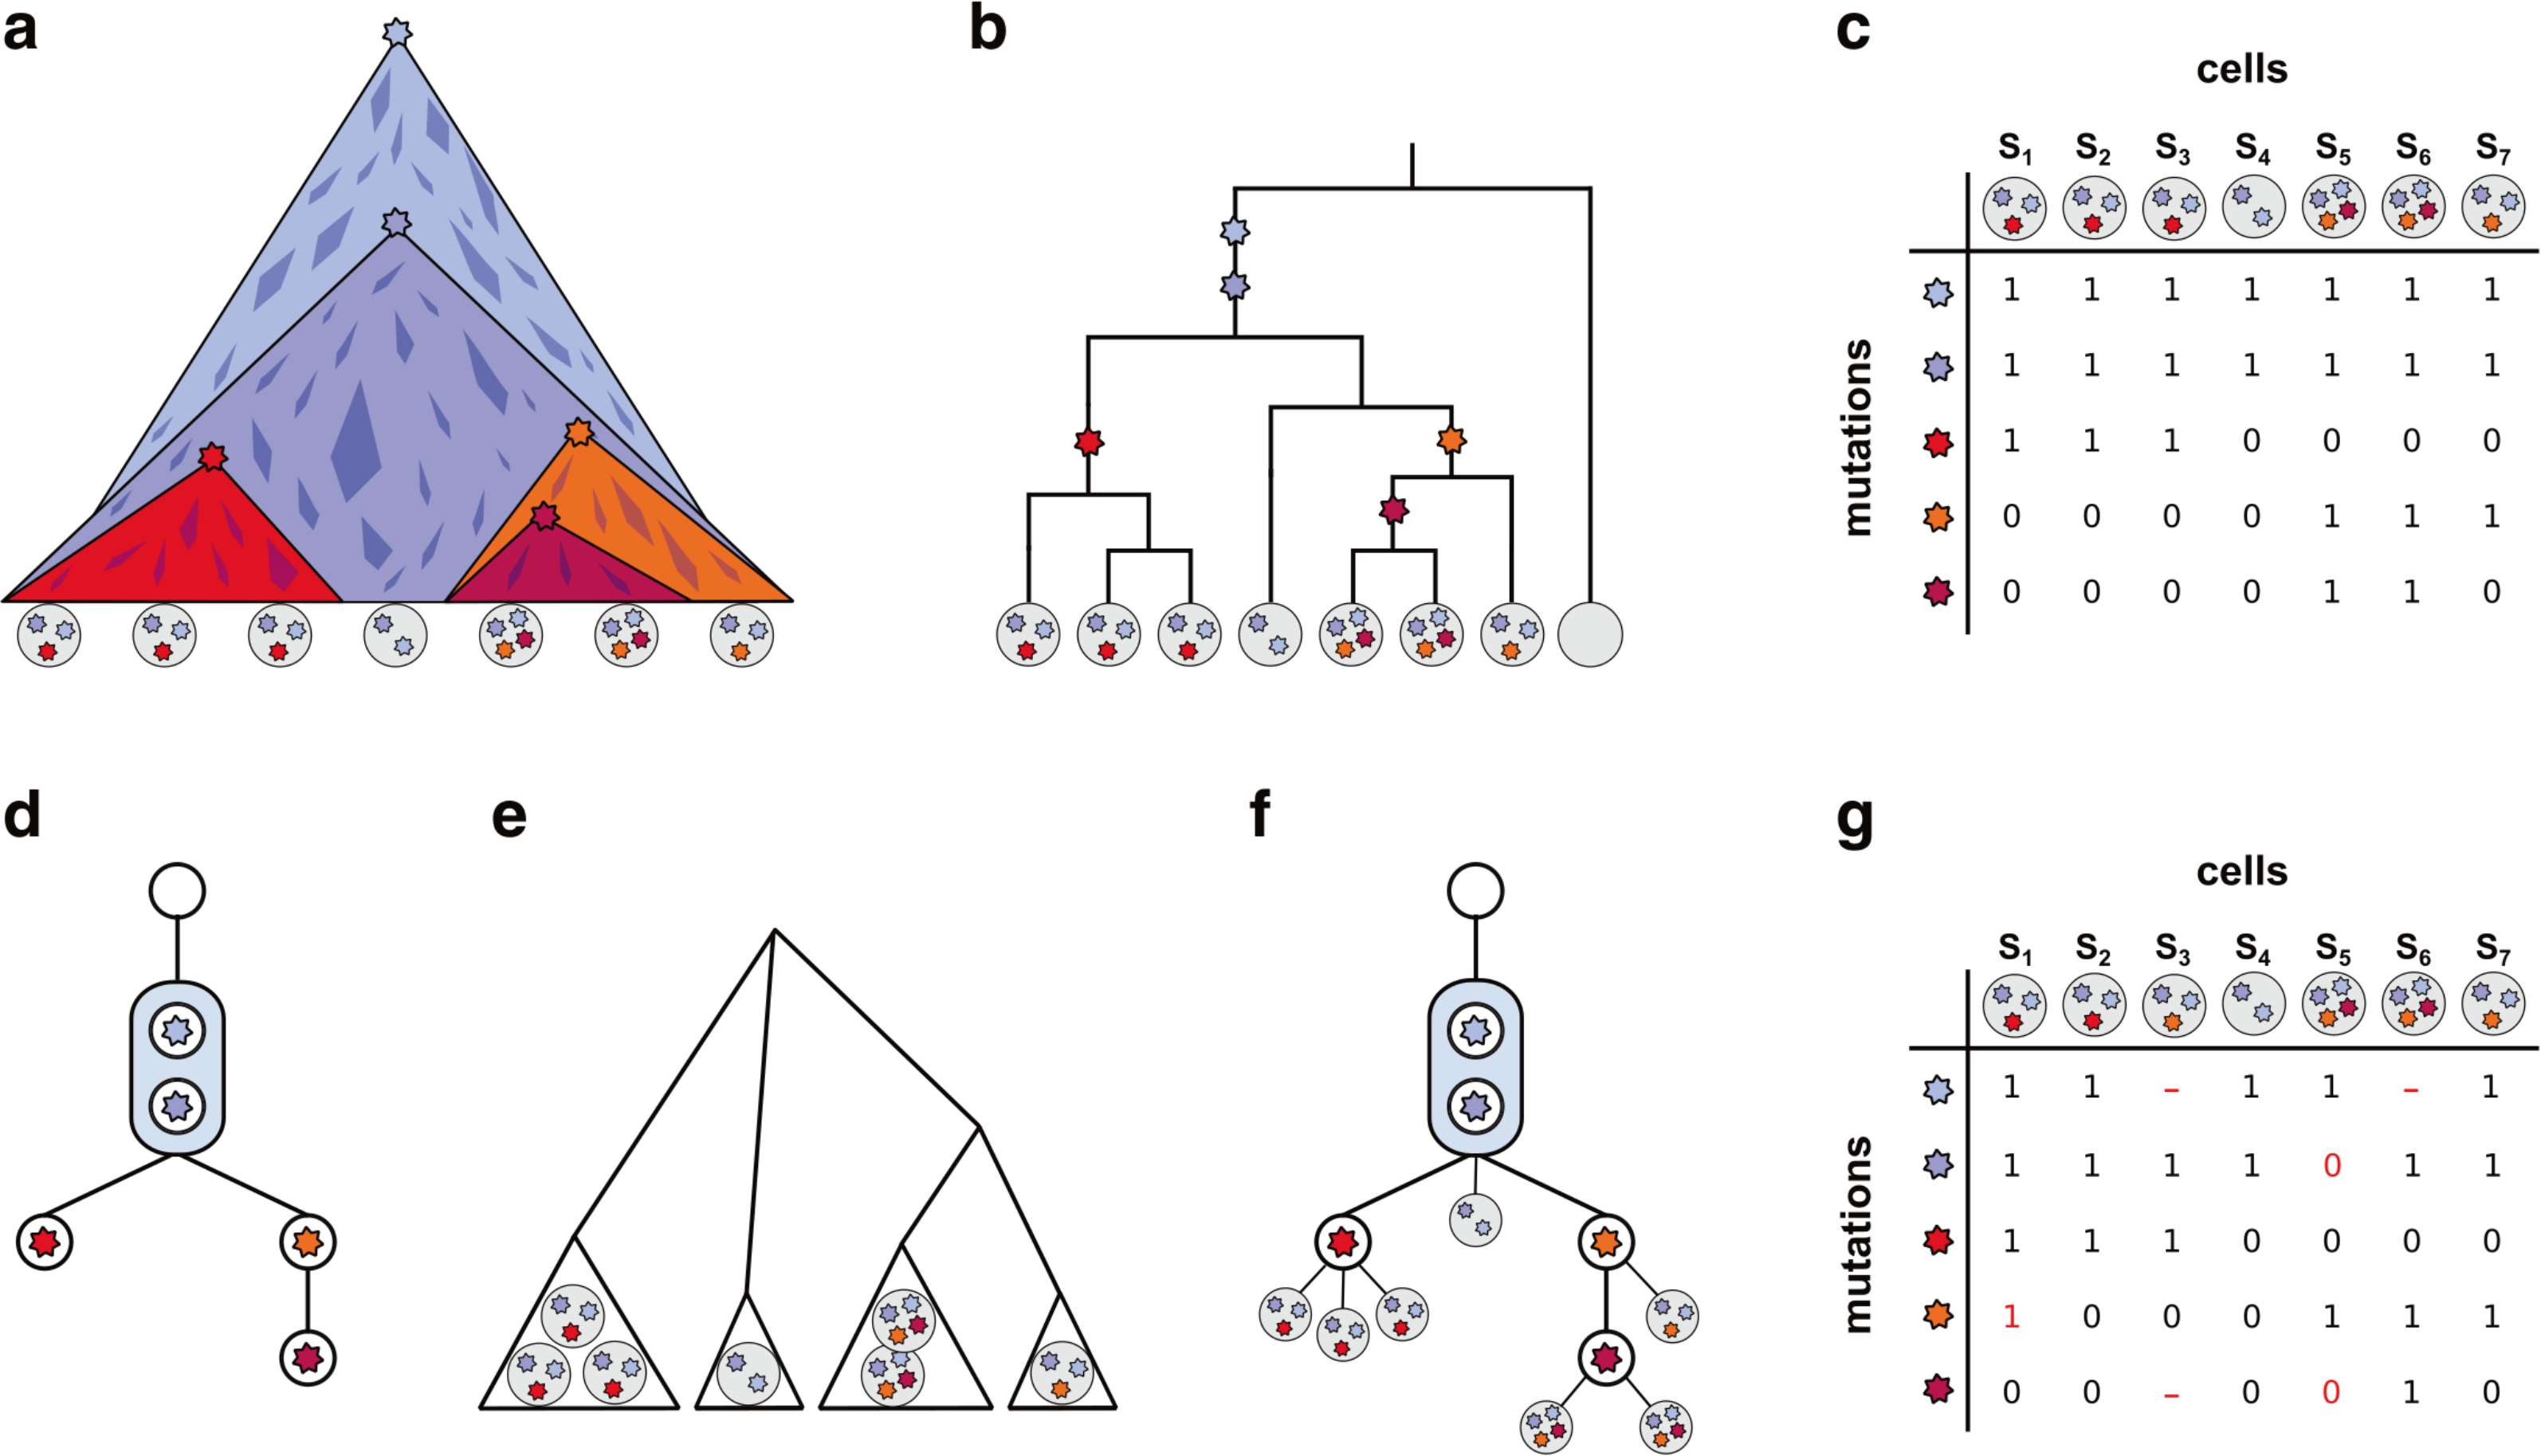
\includegraphics[width=\textwidth]{figures/example_tree.png}
    \centering
    \caption{``Tumor evolution and cell phylogeny. \textbf{a} Schematic representation of tumor evolution with time progressing downwards. Stars denote new mutations leading to subclone expansion. The quadrangles belong to minor extinct subclones with no traces in the present-day populations. The mutations founding these clones may not have induced a sufficient growth advantage to have surviving descendant cells or may have been lost by chance. The gray discs on the bottom denote single cells sequenced after tumor removal. The stars they contain indicate the mutations observed in the cell. \textbf{b} Binary genealogical tree of the sequenced cells. An empty disc represents a normal somatic cell, which is an outgroup for the tumor cells. \textbf{c} Binary mutation matrix representing the mutation status of the sequenced tumor cells. A zero entry denotes the absence of a mutation in the respective cell, while a one denotes its presence. \textbf{d} The perfect phylogeny represented as a mutation tree, the partial (temporal) order of the mutation events. Mutations are summarized in a single node when their order is unidentifiable from the sampled cells, as is the case here for the two top-most mutations with the matrix from (c). \textbf{e} Hierarchical subclone structure. Cells with identical mutation profiles cluster into subclones, which serve as taxa in this phylogenetic tree. \textbf{f} Mutation tree with single-cell samples attached. \textbf{g} Noisy mutation matrix with missing values. The red numbers indicate flipped mutation states with respect to the true mutation matrix in (c). For 0→ 1, a false positive, the mutation is called but not present in the cell. For 1→ 0, a false negative, the mutation is not called but present in the cell, most likely due to allelic dropout during the DNA amplification. The red dash indicates a missing value; it is unknown whether the site is mutated or in the normal state in this cell.'' \cite{tree2016}, Copyright (C) Katharina Jahn et al., CC-BY 4.0, screenshot and cropped.}
    \label{fig:exampletree}
\end{figure}

Figure \ref{fig:exampletree} illustrates this: We assume that mutations are introduced by a single cell and are passed down to all subclones. Among these subclones, new mutations may occur, which are passed down again. The ancestry of a cell defines its genome and we can model this ancestry with a tree: In this so-called phylogenetic tree or mutation tree, every node except for the root represents a gene that may be mutated. Then, we attach every cell to a node, which expresses that this cell has all mutations on the path from the root to its attachment point, but no others. We can then construct the true mutation matrix according to this mutation tree. If we have the probabilities for false positives and false negatives given, we can then compute the likelihood that the true mutation matrix is correct.

Jahn et al. designed \ac{SCITE} as a \ac{MCMC} algorithm to find the maximum likelihood tree. A Monte Carlo algorithm runs a random experiment that produces a possible solution to a problem and evaluates how well the generated solution solves the problem. This loop of generating and evaluating a solution is then repeated multiple times and the result is the best solution the algorithm has encountered. In theory, it would suffice if the experiment had a probability greater than zero to produce a good solution, but in order to improve the solution quality and reduce the required repetitions, one would use an experiment that produces the best solutions with a higher probability than worse solutions and that can be repeated quickly. As the name implies, \ac{MCMC} algorithms are Monte Carlo algorithms that simulate a Markov Chain to produce solutions. The advantage of using Markov Chains is that the next sample may depend on the previous one and the algorithm therefore only needs to introduce small changes to the solution. This is often faster than generating a new solution from scratch and if the current sample is already a good solution, the change may preserve some of its quality. However, the designer of a \ac{MCMC} algorithm has to make sure that the chain actually converges on the desired distribution.

\ac{SCITE}'s chain state is a mutation tree and in order to transition from one chain state to the next, a random modification is proposed to this tree. This chain would however aimlessly walk through the set of all trees and would have a low probability to encounter a maximum likelihood tree. \ac{SCITE} therefore only proposes a modification and computes its likelihood. If the modification improves the chain state's likelihood, it is always accepted as the new state of the chain, but if it does not, it may be rejected with a probability that rises with the decrease of likelihood produced by the modification.

There are multiple challenges in implementing the \ac{SCITE} algorithm for \acp{FPGA}: First of all, we require a data structure for mutation trees that allow us to easily propose, execute and evaluate state changes. Then, there is the issue of proposing modifications: This requires the generation of random numbers, and random number generators are notorious for being hard to implement correctly and efficiently. Lastly, computing a tree's likelihood is an issue too and there are the usual problems with external memory 

We faced multiple challenges during our work: First of all, we had to develop data structures and algorithms to efficiently propose, execute and evaluate state changes. Then, we had to restructure and optimize the likelihood computation method to adapt it to an \ac{FPGA}'s structure. We also faced issues with random number generation for tree move proposals since those implementations available to us have high resource and timing demands. Then, we had to optimize our IO and feedback structure to assure that the resulting chip design is always fully utilized. Lastly, we also had to verify that our implementation is indeed correct: As a randomized algorithm, there is a probability that even a correct implementation does not find the maximum likelihood tree. We therefore had to design a statistical test to compare our implementation with the reference.